\chapter{Exigences et aperçu général}
\label{chap::exigences}


\section{Rappel des exigences}

L'application va permettre d'aider les \ris à simplifier la gestion des mobilités des étudiants. L'affectation et le suivi des mobilités sont séparés en trois phases, ou étapes. 


\bigbreak

La première correspond, pour les étudiants (ou élèves dans la rapport), à la recherche de l'université de destination et au choix de leurs \voe. Ils doivent donc pouvoir accéder à la liste des écoles. Une liste de commentaires des élèves déjà partis vers ces destinations doit également être présente.

Les \ris peuvent gérer les étudiants, les écoles partenaires, les \voe des étudiants et enfin leur affectation. Les affectations peuvent être effectuées de façon manuelle, ou de façon automatique à l'aide d'un algorithme qui pourra être choisi. Lorsque chaque étudiant a une école qui lui est affectée, la deuxième phase commence.
\bigbreak

Certains documents sont nécessaires pour la mobilité. Ils devront être accessibles en téléchargement, et une génération de façon automatique peut être envisagée. Les \ris et membres du SRI (Service Relations Internationales) doivent pouvoir récupérer ces fichiers. Ils disposeront donc de certaines vues en commun avec les \ris, mais ne pourront pas valider les affectations des étudiants. Enfin, les documents devront être signés de façon électronique. La figure \ref{fig::diffRI-SRI} ci-dessous récapitule les rôles des \ris et des membres du SRI.

\begin{figure}[H]
	\centering
	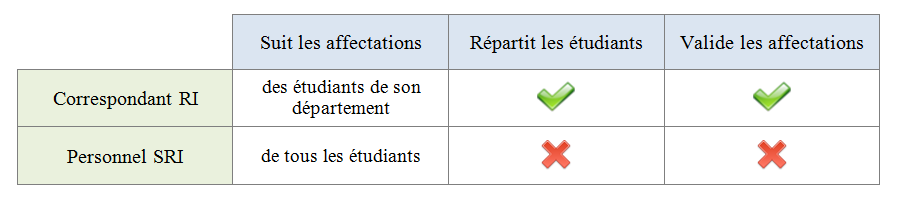
\includegraphics[scale=0.4]{roleRI-SRI.png}
	\caption{Page d'accueil pour les étudiants dans l'étape 1}
	\label{fig::diffRI-SRI}
\end{figure}
\bigbreak

La troisième et dernière phase correspond au suivi des mobilités après le départ des étudiants. Le contrat de mobilité doit pouvoir être modifié par l'élève, et les \ris doivent en être notifiés. Ils pourront ensuite valider le nouveau contrat. A la fin de la mobilité, l'étudiant pourra entrer ses notes sur le site pour le jury de fin d'année. Il pourra également laisser un commentaire sur l'université pour aiguiller les étudiants intéressés. La demande de génération de fiches de jury pourra être demandée par les \ris.


\section{Vue globale de l'application}

\begin{figure}[H]
    \centering
    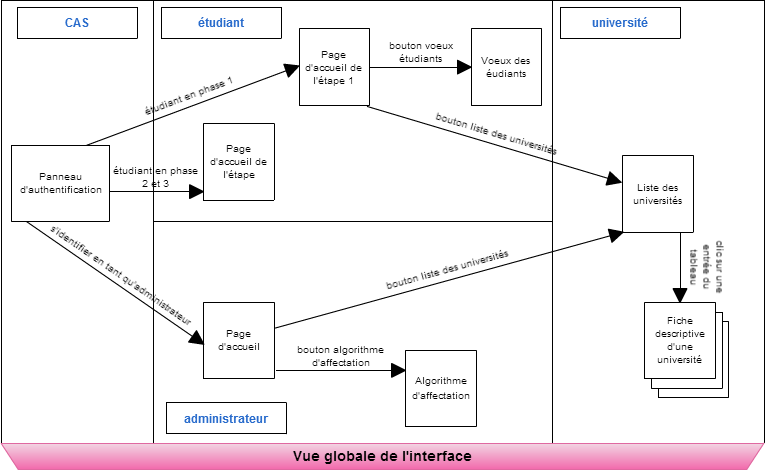
\includegraphics[angle=90,scale=0.7]{Annexe/vue_globale.png}
    \caption{Vue globale de l'interface utilisateur}
    \label{fig::vue_glob}
\end{figure}

\bigbreak

Nous avons préféré séparer dans la suite du rapport les vues, non pas selon l'ordre des phases, mais plutôt celles accessibles aux étudiants, aux administrateurs, et enfin les vues concernant les universités, qui sont communes à ces deux utilisateurs.

